%
%	WISS 2026サンプルファイル
%
%	2010/07/12 Ver 1.0 秋田 純一
%	2010/08/04 Ver 1.1 後藤 真孝
% 	2011/09/27  Ver 1.4 渡邊 恵太 (協力：五十嵐悠紀)
% 	2015/02/08  Ver 1.5 大槻 麻衣
% 	2015/07/09  Ver 1.6 大槻 麻衣（協力：三浦元喜）
% 	2016/05/26  Ver 1.7 大槻 麻衣
% 	2017/02/04  Ver 1.8 大槻 麻衣
%	2018/05/01  Ver 1.9 中村 裕美
%	2019/04/05  Ver 2.0 中村 裕美, 池松 香
%   2020/08/25  Ver 2.1 池松 香
%   2021/07/14  Ver 2.2 池松 香
%   2022/07/06  Ver 2.3 池松 香
%   2022/11/27  Ver 3.0 池松 香
%   2024/05/27  Ver 3.1 石井 綾郁
%   2025/05/30  Ver 3.2 石井 綾郁
%   2026/05/25  Ver 3.3 石井 綾郁

\documentclass[twoside]{wiss}

\usepackage{ascmac}
% \usepackage[dvips]{graphicx}
\usepackage[dvipdfmx]{graphicx} %% グラフィックエンジンをラスタにも対応させるため変更（2024/05/27: Ishii）
\usepackage{nidanfloat} %% appended in WISS2010 for Future Vision (2010/7/7:akita)
\usepackage{multicol}
\usepackage{color}
%\usepackage{color,array}
%\usepackage{boxedminipage}

%% balance.styを追加 (2012/9/27:watanabe, Igarashi)
% \usepackage{balance}    %% 最後のページの高さを揃えるために追加  (2012/9/27:watanabe, Igarashi)
%%% 最後のページの2段組の高さを揃える．\balanceを入れる．
%%% そろえたくないときは，\nobalance
%% 参考文献のバランスのとり方: flushendに変更 (2022/11/27: Ikematsu)
\usepackage{flushend}

%% urlのOverflow対策
\usepackage{url}

%% \showURLマクロの定義（jwiss.bstで使用）
\newcommand{\showURL}[1]{\url{#1}}

%% 全著者の所属が同じ場合はマークを付けない（テンプレートの指示に準拠）
\renewcommand{\affil}[1]{%
  \begingroup
    \let\footnotemark\relax
    \thanks{#1}%
  \endgroup
}

\journalhead{Shap3Base:製造容易かつカスタマイズ性・再利用性を実現する形状提示ディスプレイ用3Dプリントリニアアクチュエータ} %%%%%% ←←　著者において必ず記入すること

\begin{document}

% 登壇発表用のテンプレートではありません
\title{Shap3Base:製造容易かつカスタマイズ性・再利用性を実現する\\形状提示ディスプレイ用3Dプリントリニアアクチュエータ}
\etitle{}%2012年では英文タイトルは廃止されました．記入しないでください．
%
%注意
%
%
% WISS2016からシングルブラインドとなりました．投稿時に氏名と所属を記入してください．
\author{鈴木 太　　岩井 将行\affil{東京電機大学}}

\begin{abstract}
ピンアレイ型形状提示ディスプレイ（Shape Display）は，物理的な3D形状を動的に変形・提示可能なインタフェースとして期待されているが，
多数のアクチュエータの製造コスト，機構的複雑さによるメンテナンス性，および部品の再利用性の低さが大きな課題となっている．
本稿では，主要な伸縮構造をすべて3Dプリンタ（PLA素材）で造形し，スナップフィット機構を活用することで追加の締結部品（ネジ・ナット等）を不要としたリニアアクチュエータ「Shap3Base」を提案する．
本手法では，入手性と再利用性に優れる連続回転サーボモータと伸縮距離センサ以外の電子部品・機械部品を極力排除し，ピンセット等のみで容易に組み立て・分解可能なモジュール構造を実現した．
現段階で実現しているCADモデル上での伸縮部の太さ・長さの設計変更可能性を示すとともに，複数モジュールの試作および駆動・センシングについて述べる．
\end{abstract}

\maketitle

\section{はじめに}

デジタル情報を物理空間上に立体形状として提示する形状提示ディスプレイ（Shape-Changing Display）は，HCI分野において長年にわたり活発に研究されている．
その代表的アプローチであるピンアレイ（Pin-Array）方式は，Lumen やinFORM に代表されるように，無数のピンを垂直方向に駆動させることで2.5次元の形状を動的に生み出す．
近年のピンアレイ型形状提示ディスプレイは，単なる立体形状の提示にとどまらず，視覚情報の統合など他メディアと融合した高度な表現装置へと進化している．
しかし，その基盤となるアクチュエータの多くは専用部品や複雑な構造に依存しており，プロトタイピングにおける複製や，用途に応じた機能・パラメータの変更（カスタマイズ）には依然として障壁が存在する．
また，それら障壁を回避しながらモジュール単位での柔軟な機能付加や再利用を可能にする統合的な設計基盤には発展の余地がある．
そこで本研究では，製造容易性・カスタマイズ性・再利用性を兼ね備えた3Dプリントリニアアクチュエータ「Shap3Base」を提案する．
本システムは，汎用3Dプリンタとスナップフィット構造を活用することで，工具レスでの組み立て・解体を可能にし，様々な機能要素の付加や仕様変更に柔軟に対応する．
本稿では，本システムの設計コンセプトとパラメータ変更による拡張性，および今後の課題について報告する．
\cite{rekimoto2000}

\section{関連研究}

\subsection{ピンアレイ型ディスプレイの駆動機構}
ピンアレイ型形状提示ディスプレイにおいて，各ピンの位置を正確に制御・保持する手法としてリードスクリュー（送りねじ）機構が頻繁に用いられている．
しかし，ピンごとに独立した駆動部を多数複製する構成は部品点数を大幅に増大させ，コストの増加やシステム全体の故障率を高める直接的な原因となる．
また，inFORM や Elevate に代表される先行研究では，高い機能性を実現する一方で，複雑な金属加工部品や独自のロック機構，専用設計の回路基板などが採用されている．
近年では入手性の高い3Dプリンタを利用した装置製作も普及しつつあるが，それらの多くは特定の単一目的のための専用装置として開発される傾向が強く，
個人研究者やプロトタイピング用途における装置の複製や拡張を行う上では，製造の容易性とメンテナンス性や再利用性には探求の余地がある．

\subsection{形状提示でのモジュール化のアプローチ}
ピンアレイ型ディスプレイでは，ピン（アクチュエータ）に対して液晶ディスプレイや可動膜などの機能要素を付加することで，物理形状以外の表現能力を複合的に拡張する試みが広く行われている．
ShapeClip や CommuTiles に示されるように，ディスプレイを構成する画素的要素を独立したユニットとしてモジュール化するアプローチは，システムの高いスケーラビリティや多様な応用可能性をもたらす．
しかし，こうしたユニット化による柔軟性を担保しながら，用途に応じて付加したい機能要素やそれに適した駆動パラメータを自由に構成・選択できるような，モジュールレベルでの高カスタマイズ性を備えた統合的な設計基盤は十分に提供されていない．


\section{"Shap3Base"の設計思想と実装}
前述の関連研究で示されたピンアレイ型形状提示ディスプレイの装置製造及び拡張の容易性に関する課題を踏まえ，本研究では以下の設計思想に基づき，3Dプリントリニアアクチュエータ「Shap3Base」を開発した．
\subsection{3Dプリントによる製造の容易化}
各構造・部品間の結合には，PLA素材の弾性変形を利用した「スナップフィット」構造を多く採用した．その結果，ほとんどの部品を一括で3Dプリントし，
金属ネジやインサートナットを用いずにサポート材の除去用ピンセットのみで組み立て可能となった．
それにより，ネジ部品や送りねじ等の発注待ちによる開発遅延を排除し，実験室環境での試作サイクル（高速プロトタイピング）の加速に貢献する．
なお，より強固な結合が要求される用途のために，熱圧入によるインサートナットを組み込めるネジ留め穴もオプションとして設計に含まれている．

\subsection{2段並列送りねじ機構による全長短縮}
従来の1段送りねじ機構では，収納時の全長が伸長時の半分以上となり，装置全体の奥行きが大型化する課題があった．
本研究では，独自のネジピッチ，リード角度，ハメ合い公差を検証して決定した3Dプリント製送りねじを採用した．
さらに，2つの送りねじ機構をアクチュエータ内部に並列して統合する「2段伸縮機構」を開発した（図2）．
これにより，伸長時の全長が約200mm以上の場合において，収納時の全長を伸長時の半分以下に収めることに成功した．
また，伸縮部を細く抑えたい用途向けには，構造が簡易な「1段伸縮機構」も選択可能としている．


\subsection{電子部品の選定と再利用性}
\begin{itemize}
    \item \textbf{駆動モータ}: 入手性が高く小型軽量な連続回転サーボモータ（SG90R系）を採用した．本モータの発生トルクは人間が手で動作を停止させられる程度であり，ピンアレイディスプレイの誤作動時における安全性の観点からも適している．
    \item \textbf{伸縮距離センサ}: Dedicated基板を不要とし再利用性を高めるため，ToF測距センサ（M5Stack用 VL53L1X）を採用した．光学式測距のため，ロータリーエンコーダと異なり，停電や電源断が発生しても外部メモリなしで即座に絶対位置（伸縮距離）を再取得できるメリットを持つ．
\end{itemize}

\section{カスタマイズ性の検討と試作}
現段階の実装において，全パラメータを網羅した物理試作の評価までは至っていないものの，
Fusion360（CAD）上でのパラメータ変更およびBambulab製3Dプリンタ（H2S, P1S）によるPLAフィラメントを用いた部品出力により，造形適合性を検証している．
CADモデルの検討により，以下のカスタマイズが可能であることを確認している．
\begin{enumerate}
    \item \textbf{伸縮段数の変更}: 伸縮距離を重視する2段機構と，断面外形を細くして高密度配置を優先する1段機構の切り替え．
    \item \textbf{パラメータ可変}: 用途に応じた全長，伸縮距離，伸縮部外径の変更．
    \item \textbf{先端アダプタの換装}: 先端部に小型ディスプレイ（可動ディスプレイボクセル等）や各種センサ，物理UIパーツを結合するための共通スナップフィット形状の付加．
\end{enumerate}



\section{制御構成例}
本アクチュエータは汎用的なインターフェース（モータ：PWM 3線式，センサ：I2C/Grove）を採用している．
今回のプロトタイプ実装例では，マイコンに「M5StickC Plus」，I2C拡張ユニット「Unit PaHub」，モータドライバ「8ch Servo Driver Unit」を組み合わせ，
スイッチング電源から給電することで，4基のアクチュエータを個別に伸縮制御する環境を構築した．

\section{現在の課題及び考察}
プロトタイプの予備動作実験を通じて，以下の課題が明確となっている．
\subsection{伸縮距離センサの個体差と測定精度}
ToFセンサ（VL53L1X）は数mm精度での測距が可能である一方，個体差による数mmの測定ずれが生じる．
これに対しては，起動時やアセンブリ時にソフトウェア側でルックアップテーブルを作成する等のキャリブレーション処理が必要である．

\subsection{出力トルクと伸縮速度の限界}
構造的には垂直荷重や圧縮に耐性があるが，SG90Rサーボモータの出力制限により，重い物体を持ち上げるトルクや俊敏な伸縮速度が不足する場合がある．
アクチュエータ内部に小型ギアボックスを仕込む構造や，高出力モータへ換装できるモジュール構造の導入を検討する．

\subsection{アクチュエータ外径と配置密度のトレードオフ}
高密度なピンアレイ配置（先端的な高密度ピンディスプレイ）を実現するには，現在の軸太さはやや大きい．
これは汎用のSG90RモータとToFセンサの物理サイズに起因する．
専用基板やさらに超小型のモータを採用すれば細径化は可能だが，本研究の主眼である「製造の容易さ」「低コスト」「部品の再利用性」とのトレードオフとなるため，
目的に応じた構造分離（1段化やモジュール切り替え）で対応すべきと考える．

\section{おわりに}
本稿では，製造容易性・カスタマイズ性・再利用性を目的とした形状提示ディスプレイ用3Dプリントリニアアクチュエータ「Shap3Base」を提案した．
主要な伸縮部をPLA素材の3Dプリントとスナップフィット構造で構築し，2段並列送りねじ機構により収納長の大幅な短縮を達成した．
また，市販のサーボモータとToFセンサを非破壊で容易に脱着できる構造により，高い再利用性と安全性を担保した．


今後は，出力や動作精度の定量的な性能計測を実施するとともに，キャリブレーション手法の確立を進める．
さらに，本アクチュエータ基盤上に視覚提示素子や他センサを統合し，ピンアレイと多様なHCI技術が融合した新たなメディア装置の実現に向けた応用開発を推進する．






%%
%%	参考文献
%%
% \begin{thebibliography}{1}

% \bibitem{wiss} WISSホームページ.  http://www.wiss.org/.

% \bibitem{aoki1999} H.~Aoki, B.~Schiele, and A.~Pentland.  Realtime
% Personal Positioning System for Wearable Computers.  In
% \emph{Proceedings of the 3rd IEEE International Symposium on Wearable
% Computers}, pp. 37--43, 1999.

% \bibitem{rekimoto2000} 暦本 純一.  まえがき：WISS2000について.  インタラ
% クティブシステムとソフトウェアVIII, pp. i--ii. 近代科学社, 2000.

% \end{thebibliography}



% \balance %最後の高さを揃えるために必要 (2012/9/27:watanabe, Igarashi)
% ※ \cite が1つも無い状態で \bibliography を有効にすると，参考文献が空になり
%    「missing \item」エラーでコンパイルが止まる．参考文献を入れるときは，
%    本文中に \cite{キー} を書き，下の2行を有効化する．
\bibliographystyle{jwiss}
\bibliography{sample}



%%%%%%%%%%%%%%%%%%%%%%%%%%%%%%%%%%%%%%%%%%%%%%%%%%%%%%%%%%%%%%%%%%%%%
%%%%%%%%%%%%%%%%%%%%%%%%%%%%%%%%%%%%%%%%%%%%%%%%%%%%%%%%%%%%%%%%%%%%%
%% WISS2012では，「未来ビジョン」は以下のように，本文と同様の2段組形式で記載する．
%% 図を用いても良いが，枠のサイズ(縦93mm)を変更してはならない．
%% （WISS2010では，縦118mmでしたのでご注意下さい）

\begin{figure*}[!b]
\setlength{\unitlength}{1mm}\fboxrule=0.5pt

\vspace{-93mm} %% 未来ビジョンの枠が下がってしまうのを防ぐ WIS2012 カメラレディテンプレで追加  (2012/9/27:watanabe, Igarashi)

% 未来ビジョンの枠の描画
\begin{center}
\framebox[0.95\textwidth]{
\begin{minipage}{0mm}\begin{picture}(0,91)(0,0)\end{picture}\end{minipage}
}
\end{center}
\vspace*{-93mm}	% 未来ビジョンの枠の縦幅分だけ戻す

% 未来ビジョンの内容
\newbox\FUTURE
\setbox\FUTURE=\vbox{
\begin{minipage}[b]{0.9\textwidth}
\begin{multicols}{2}	% 二段組にする
\section*{未来ビジョン}
\setlength{\parindent}{10pt}	% 段落先頭の字下げ

% % % % % % % % % % % % % % % % % % % % % % % % % % % % % %
%	   未来ビジョンは，下記に記入して下さい		  %
% % % % % % % % % % % % % % % % % % % % % % % % % % % % % %

\vspace*{-1mm}

% フォントサイズ指定
\normalsize
%\large
%\small\setlength{\baselineskip}{12pt}
%\footnotesize\setlength{\baselineskip}{12pt}

(本行を含む下記の説明を削除してから，記入すること．)

未来ビジョンについては，必須とせず任意とする．論文本体とは別
に，「この研究はどういう未来を切り拓くのか」について，著者の視点からア
ピールしたい点があれば，このような欄を設けて設けて自由に議論してよい．
例えば，「こういう未来社会が到来して欲しいから，我々の研究でこう貢献
していきたい」，「主張が大きすぎて本文中では書きにくかったが，この研究
は，実はこういう気持ちで研究している」，「現在の実装では，小さいトピック
であるかのように誤解を招きやすいが，本当はこういう大きなことを狙って，そ
の第一歩として研究に取り組んでいる」のように，研究の未来，魅力を語る場と
して利用できる．大きさや形状はこのサンプルを目安とするが，この枠内であればある程
度改変してもよいものとする．

てすとてすとてすとてすとてすとてすとてすとてすとてすとてすと．てすとてすとてすとてすとてすとてすとてすとてすとてすとてすと．てすとてすとてすとてすとてすとてすとてすとてすとてすとてすと．てすとてすとてすとてすとてすとてすとてすとてすとてすとてすと．てすとてすとてすとてすとてすとてすとてすとてすとてすとてすと．てすとてすとてすとてすとてすとてすとてすとてすとてすとてすと．てすとてすとてすとてすとてすとてすとてすとてすとてすとてすと．
%% 文章を補う図表を利用してもよい．
\vspace*{5mm}
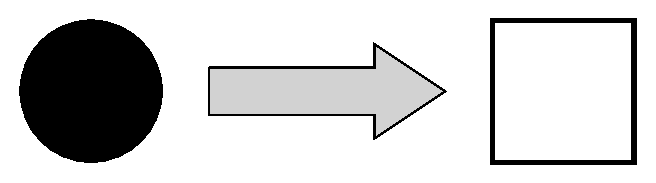
\includegraphics[width=0.95\columnwidth]{vision.eps}
% % % % % % % % % % % % % % % % % % % % % % % % % % % % % %
%	   未来ビジョンは，上記に記入して下さい		  %
% % % % % % % % % % % % % % % % % % % % % % % % % % % % % %

\end{multicols}
\end{minipage}
}

% 未来ビジョンの内容の描画
\newlength{\FUTUREHT}
\setlength{\FUTUREHT}{\the\ht\FUTURE}	% 未来ビジョンの内容の縦幅保存
%\typeout{\the\wd\FUTURE}
%\typeout{\the\ht\FUTURE}
\hspace*{0.045\textwidth}	% 未来ビジョンの内容の横位置調整
\box\FUTURE
%\typeout{\the\FUTUREHT}
\vspace*{-\the\FUTUREHT}	% 未来ビジョンの内容の縦幅分だけ戻す
\vspace*{-10.9mm}		% 微調整

% 未来ビジョンの枠の領域の再確保（これがないと枠が下に沈み込む）
\begin{center}
\fboxrule=0pt
%\fboxrule=2pt	% デバッグ用: コメントアウトをやめて，同じ位置に枠が出るか？
\framebox[0.9\textwidth]{
\begin{minipage}{0mm}\begin{picture}(0,91)(0,0)\end{picture}\end{minipage}
}
\end{center}
\end{figure*}

%%%%%%%%%%%%%%%%%%%%%%%%%%%%%%%%%%%%%%%%%%%%%%%%%%%%%%%%%%%%%%%%%%%%%
%%%%%%%%%%%%%%%%%%%%%%%%%%%%%%%%%%%%%%%%%%%%%%%%%%%%%%%%%%%%%%%%%%%%%
\end{document}
